%TODO: Chapter needs to be improved a lot
\documentclass[11pt,compress,t,notes=noshow, aspectratio=169, xcolor=table]{beamer}

\usepackage{../../style/lmu-lecture}
% Defines macros and environments
 
\usepackage[export]{adjustbox}
\usepackage[most]{tcolorbox}

\newtcolorbox{BlueBox}[2][]{%
   enhanced,
   colback   = blue!5!white,
   colframe  = blue!65!black,
   arc       = 1mm,
   outer arc = 1mm,
   fonttitle = \Large\slshape\textbf,
   center title,
   title     = #2,
   #1}

\tikzset{main node/.style={rectangle,draw,minimum size=1.2cm, minimum width=3cm,inner sep=4pt},}

\title{Interpretable Machine Learning}
% \author{LMU}
%\institute{\href{https://compstat-lmu.github.io/lecture_iml/}{compstat-lmu.github.io/lecture\_iml}}
\date{}

\begin{document}

\newcommand{\titlefigure}{../01_intro/figure/open_blackbox}
\newcommand{\learninggoals}{
\item General pitfalls of interpretation methods
\item Practices to avoid pitfalls}

\lecturechapter{Pitfalls and Best Practices}
\lecture{Interpretable Machine Learning}
%
%

% \begin{frame}[t]{Pitfalls and Best Practices~\citebutton{Molnar et. al (2021)}{https://arxiv.org/abs/2007.04131v2}}

% \begin{itemize}[<+->]
%     \item \textbf{Proper training and evaluation}:
%     To gain insights into data generating process, deployed model should at least generalize well to unseen data (garbage in, garbage out)
%     %Model interpretation is only as good as the underlying model (garbage in, garbage out).
%     \item \textbf{Avoid unnecessary complexity}: Prefer simple interpretable models and use them as baseline
%     \item \textbf{Quantify uncertainty}: Interpretation methods are often (statistical) estimators \\
%     $\leadsto$ Beware of uncertainty, we may need confidence intervals
%     %To avoid interpretation of noise, include uncertainty estimates for the interpretations, e.g.,  confidence intervals for feature importance.
%     \item \textbf{Careful with causality}:
%      Do you want to understand the model or the nature of DGP?\\
%      $\leadsto$ Your goal should guide the choice of interpretation method
%      %Causal interpretation requires assumptions about relationships in the data and a corresponding model considerations (e.g., including confounders into the model).
%     \item \textbf{Consider dependencies}: Some interpretation methods suffer when features are dependent\\
%     $\leadsto$ Check presence of dependencies and use suitable methods
%     \item \textbf{Beware of simplifications}:
%     % Interpretation methods map complex models to low-dim. explanations
%     % Interpretation methods
%     Mapping of complex models to low-dim. explanations\\
%     $\leadsto$ Information loss, e.g., some interpretation methods hide interactions
% \end{itemize}

% \end{frame}

\begin{frame}{Sources of pitfalls~\citebutton{Molnar et. al (2021)}{https://arxiv.org/abs/2007.04131v2}}

\begin{center}
    %\textbf{Data analysis process}\\
    \quad \\ \vspace{0.5cm}
    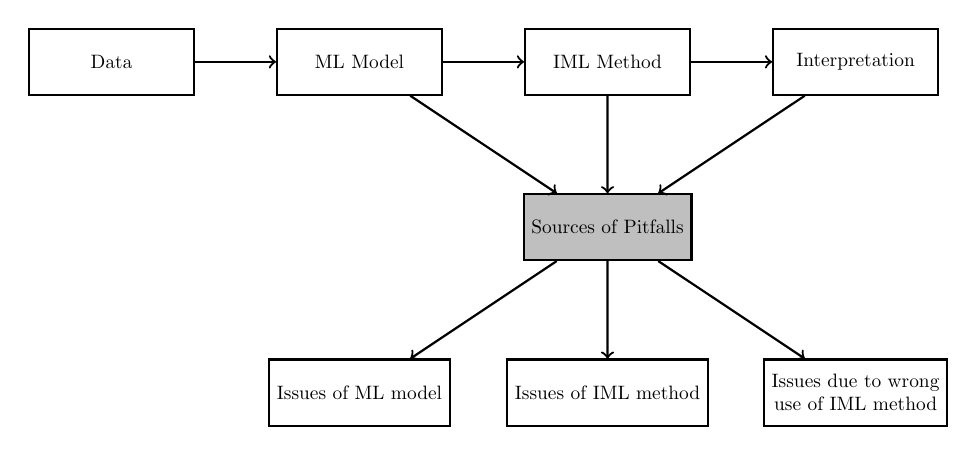
\begin{tikzpicture}[every path/.style={->,line width=0.35mm,thick},
                            every label/.append style={align=left, font=\footnotesize, text width=4cm},
                            scale=0.7, transform shape]
            \node[main node] (1) { Data };
            \node[main node] (2) [right of=1, node distance=4.5cm] { ML Model };
            \node[main node, right of=2, node distance=4.5cm] (3) { IML Method };
            \node[main node, right of=3, node distance=4.5cm] (4) { Interpretation };
            \node[main node, below of=3, node distance=3cm, fill = lightgray] (5) { Sources of Pitfalls };
            \node[main node, below of=2, node distance=6cm] (6) { Issues of ML model };
            \node[main node, below of=3, node distance=6cm] (7) { Issues of IML method };
            \node[main node, below of=4, node distance=6cm, align = center] (8) { Issues due to wrong \\ use of IML method };
            
            \draw (1) -- (2);
            \draw (2) -- (3);
            \draw (3) -- (4);
            \draw (2) -- (5);
            \draw (3) -- (5);
            \draw (4) -- (5);
            \draw (5) -- (6);
            \draw (5) -- (7);
            \draw (5) -- (8);
        \end{tikzpicture} 
\end{center}
\end{frame}


\begin{frame}{Issues of ML model~\citebutton{Molnar et. al (2021)}{https://arxiv.org/abs/2007.04131v2}}
    \begin{itemize}
        \item \textbf{Proper training and evaluation}: To gain insights into DGP, deployed model should generalize well to unseen data (garbage in, garbage out)\\
        \only<2->{\textit{Example}: $X_1, X_2, X_3 \sim Unif(-3,3)$ with $Y = X_1^2 +X_2 - 5X_1X_2 + \epsilon$, $\epsilon \sim \mathcal{N}(0, 5)$\\
        Figure: PDP of DGP (true effect), linear regression model (underfitted), random forest (overfitted), and SVM with radial basis kernel (good fit).
        \begin{center}
            \includegraphics[width=0.8\textwidth]{../01_intro/figure/pitfall1.png}
        \end{center}}
        \item<3> \textbf{Avoid unnecessary complexity}: Prefer simple interpretable models and use them as baseline, move to more complex models if performance not sufficient
    \end{itemize}
\end{frame}


\begin{frame}{Issues of IML method~\citebutton{Molnar et. al (2021)}{https://arxiv.org/abs/2007.04131v2}}
    \begin{itemize}
        \item \textbf{Consider dependencies}: Some interpretation methods have issues in case of dependent features \\
        $\leadsto$ Check presence of dependencies and use suitable interpretation methods\\
        \only<2->{\textit{Example:} Explanations may rely on unreliable pred. where model extrapolated}
    \end{itemize}
    \only<2->{\centerline{\includegraphics[width=0.9\textwidth]{../01_intro/figure/extrapolation}}}
    \only<3->{\begin{columns}[T, totalwidth=\textwidth]
    \begin{column}{0.6\linewidth}
	    \begin{itemize}
        \item \textbf{Beware of simplifications}:
        Mapping of complex models to low-dim. explanations\\
        $\leadsto$ Information loss, e.g., some interpretation methods hide interactions or heterogeneous effects (Figure: PDP and ICE Curves)
    \end{itemize}
	\end{column}
	\begin{column}{0.4\linewidth}
    \centerline{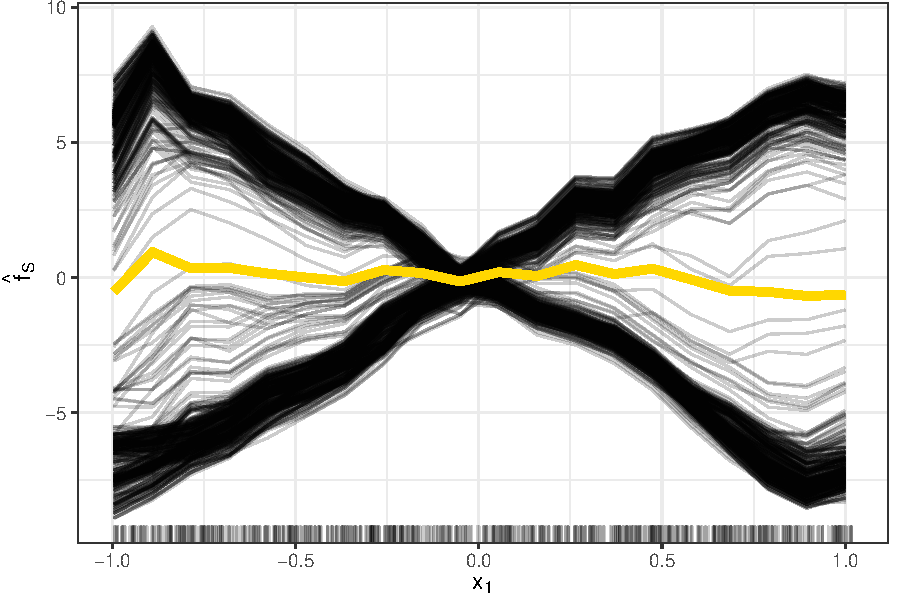
\includegraphics[width=0.8\textwidth]{../03_feature-effects/figure/pdp_xor.pdf}}
    \end{column}
	\end{columns}}
    
\end{frame}








\begin{frame}{Interpretations with Dependent Features}
\begin{itemize}

% \item Be clear about interpretation goal: Explain model or underlying relationship in data?
% %We need to differentiate between interpretations of a model or reality
% \\
% $\leadsto$ Latter might be distorted by modeling fallacies, 
% e.g., 
% %due to bad data quality, 
% under- and overfitting or extrapolation

%\pause
\item Highly correlated features contain similar information \\
$\leadsto$ Model might pick only 1 feat. (regularization), even if it is causally irrelevant \\
%Some models might use only one correlated feature (even if it is causally not relevant)
%Can confuse a model so that only one correlated feature is used (even if it is not relevant) \\
$\leadsto$ Produced explanations can be misleading (true to model, but not to data) % generating process
\\
$\leadsto$ E.g., different interpretable models produce different results
%$\leadsto$ Different IML models often produce different results in these situation, and not always trivial to understand which / why 
%Even for two causally and equally relevant correlated features it is not guaranteed that their explanations will be similar
% \pause
% \item Assume two causally and equally relevant but highly correlated features \\
% $\leadsto$ One might expect that their explanations (e.g., feature importance) will be similar \\
% %One might expect that explanations of two correlated features (e.g., feature importance) are similar as they share similar information \\
% $\leadsto$ Generally not true as the model can learn different relationships


% \begin{tikzpicture}[remember picture,overlay,shift=(current page.center)] %opacity=.2,text opacity=1
% \node[fill=white, opacity=1,text opacity=1] at (current page.center) {\includegraphics[width=0.6\textwidth]{figure/ridge_lasso}};
% \end{tikzpicture}
\pause

% \only<3>{
%  \begin{BlueBox}{Example}
%   \begin{columns}[c, totalwidth=\textwidth]
% \begin{column}{0.5\textwidth}
% \includegraphics[trim=0px 110px 30px 0px, clip, width=\textwidth]{figure/ridge_lasso}
% \end{column}
% \begin{column}{0.5\textwidth}
% \includegraphics[trim=0px 0px 0px 115px, clip, width=\textwidth]{figure/ridge_lasso}
% \end{column}
% \end{columns}}
% \end{BlueBox}
% }

%\only<3>{
%\colorbox{blue!20}{
%\includegraphics[trim=0px 0px 0px 115px, clip, width=.55\linewidth]{figure/ridge_lasso}}
%\begin{columns}[T, totalwidth = \textwidth]
%    \begin{column}{0.5\textwidth}
%\scriptsize
\item \textbf{Example:} Simulate 100 obs. from DGP $Y = 0.2 (X_1 + \dots + X_5) + \epsilon, \epsilon \sim N(0,1)$

\centerline
%    \end{column}
%    \begin{column}{0.5\textwidth}
        
\begin{itemize}
    \item $X_1, \dots, X_4 \sim N(0, 2)$ (uncorrelated)
    \item $X_5 = X_4 + \delta, \delta \sim N(0, 0.3)$ $\Rightarrow \rho(X_4, X_5) = 0.98$ (highly correlated)
    \item LASSO: Shrinks coef. of $X_5$ to zero, coef. of $X_4$ about $1.5 \times$ higher
    \item Ridge: Similar coef. for $X_4$ and $X_5$ for higher lambda
\end{itemize}
%    \end{column}
%\end{columns}

\end{itemize}

\end{frame}



\begin{frame}{Extrapolation due to Dependencies}
%\begin{center}
\centerline{\includegraphics[width=\textwidth]{../01_intro/figure/extrapolation}}
%\end{center}

\begin{itemize}
%\itemsep1em
\item Many interpretation methods are based on
%rely on varying feature values and create
artificially created data points \\
$\leadsto$ Many points lie in low-density regions if features are dependent\\
$\leadsto$ Predictions in such regions have high uncertainty\\ % in regions with no or few training data
$\leadsto$ Explanations can be biased if they rely on pred. where model extrapolated\\
\pause
%\item 
%\item Essentially, we are interested in the prediction uncertainty\\
%, i.e., the less the training data on a feature subspace, the higher the prediction uncertainty.
%$\leadsto$ Models are rarely able to quantify uncertainty of predictions %Models are rarely capable of quantifying prediction uncertainty
\item There is no definition of when a model extrapolates and to what degree \\
$\leadsto$ Severity of extrapolation depends on model %, some extrapolate more than others 
\\
$\leadsto$ Density of train data may helps identify regions where extrapolation is likely \\
\phantom{$\leadsto$} But: Density estimation in many dimensions is often infeasible
%$\leadsto$ Some models might extrapolate more than others
%\item Density of training data might serve as proxy to identify regions where extrapolation is likely\\
%$\leadsto$ Density estimation in many dimensions is often infeasible
\end{itemize}

\end{frame}









\begin{frame}{Issue: Wrong use of IML method~\citebutton{Molnar et. al (2021)}{https://arxiv.org/abs/2007.04131v2}}
    \begin{itemize}
        \item \textbf{Quantify uncertainty}: Interpretation methods are often (statistical) estimators \\
        $\leadsto$ Beware of uncertainty, we may need confidence intervals\\
        \only<2->{\textit{Example:} Left plot (IML method output) misleading compared to fitted models in right plot \\
        \centerline{\includegraphics[width=0.9\textwidth]{../01_intro/figure/pitfall5}}}
        \item<3> \textbf{Careful with causality}:
        Want to understand the model or the nature of DGP?\\
        $\leadsto$ Goal should guide the choice of interpretation method
    \end{itemize}
\end{frame}


\endlecture
\end{document}
